\section{An Overview of OpenMP's Evolution}
\label{sec:evolve}

As hardware capabilities and the need to support a wider range of algorithms
grew, the complexity of the specification expanded.  We can see this in
Figure~\ref{omppcount} where the pages of the specifications (not including
appendices or indices) are listed.   The initial OpenMP specification (OpenMP
Version 1.0 for Fortran) was around 45 pages long.  The  latest specification
(OpenMP 4.5 for Fortran, C and C++)  has over 300 pages.

We also see the evolution of language support in OpenMP in
Figure~\ref{omppcount}.  Prior to version 2.5 of the specification released in
2005, an OpenMP specification was specialized to a particular language.   This
made writing the text of the specification much easier, but given that most of
the people working on the Fortran specifications also worked on the C/C++
specifications, we could not run the two language committees in parallel.  This
led to long delays between updated specifications such as the almost 4 year
delay between OpenMP 1.0 for C/C++ and OpenMP 2.0 for C/C++.  The process of
merging the two languages into a single specification was a much larger
undertaking than any of us expected at the time and required us to go back and
recast the core abstractions behind OpenMP much more carefully so they would
apply across languages.  The resulting OpenMP version 2.5 specification took
three years to create.

OpenMP is no longer a simple API the full breadth of which can be learned in
less than a day.  Features were added to address non-uniform memory
architectures, more complex concurrency control, irregular algorithms,
accelerators, and much more.   Specification do not grow due to a lack of
discipline by the designers.  They grow as users demand new features and
hardware changes.  In that light, an almost seven-fold increase in size over the
course of almost 20 years is not surprising.

\begin{figure}
  \centering
  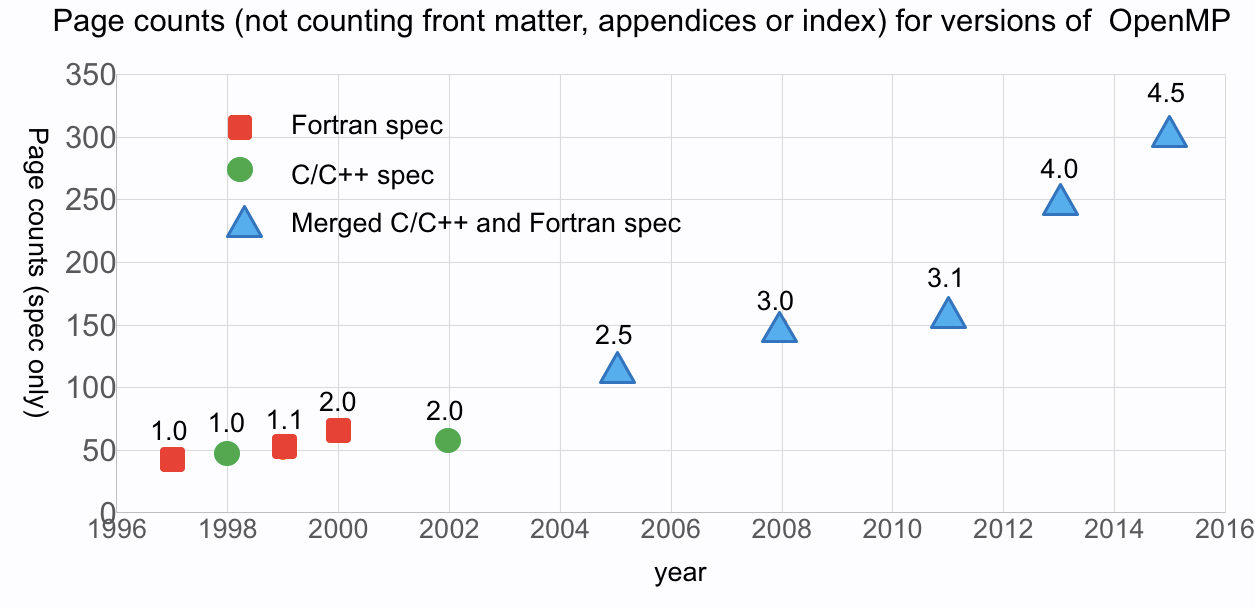
\includegraphics[width=3.4in]{pics/opcounts.png}
  \caption{OpenMP specification release dates, page counts and language bindings.}
  \label{omppcount}
\end{figure}


